\documentclass[12pt,a4paper]{article}
\usepackage[utf8]{inputenc}
\usepackage[portuguese]{babel}
\usepackage[T1]{fontenc}
\usepackage{amsmath}
\usepackage{amsfonts}
\usepackage{amssymb}
\usepackage[left=3.0cm,right=3.0cm,top=3.5cm,bottom=2.5cm]{geometry}
\usepackage{makeidx}
\usepackage{graphicx}
\usepackage{fancyvrb}

\usepackage{placeins}

\setcounter{tocdepth}{4}
\setcounter{secnumdepth}{4}

\usepackage{sectsty}
\allsectionsfont{\normalfont\scshape}

\begin{document}

\begin{titlepage}

\begin{center}

\textbf{UNIVERSIDADE FEDERAL DE SÃO CARLOS\\CAMPUS SOROCABA\\\vspace{3cm} BACHARELADO EM CIÊNCIA DA COMPUTAÇÃO\\\vspace{3cm}BANCO DE DADOS\\
Prof. Sahudy Montenegro González\\\vspace{3cm}
PROJETO PRÁTICO - FASE INTERMEDIÁRIA I/II\\\vspace{0.5cm}
TEMA 12 - Banco de Questões de Disciplinas\\\vspace{4.0cm}
Bianca Gomes Rodrigues\\
Pietro Zuntini Bonfim\\
\\\vspace{4cm}
Sorocaba-SP\\2018}

\end{center}

\end{titlepage}

\pagebreak
\renewcommand*\contentsname{Índice}
\tableofcontents
\pagebreak

\section{Descrição do Mini-Mundo}

Um dos problemas que muitos professores e alunos enfrentam na Universidade é não ter um mecanismo de aprendizado eficiente. Para tal, seria eficiente e interessante criar um sistema de gestão para armazenar questões de uma disciplina, de modo a auxiliar tanto os alunos quanto os professores, facilitando o controle do professor e o aprendizado e fixação dos alunos.\par
Através do sistema, é possível que o aluno tenha acesso à um banco de questões fornecido pelo professor de uma determinada disciplina, e possa estudar através deste para provas e outras avaliações respondendo às perguntas fornecidas e recebendo feedback de quantas questões respondeu e quantas acertou. Consequentemente, o professor também conseguiria ter controle do desempenho do aluno ao longo do semestre.\par

\section{Projeto Conceitual}

Começaremos descrevendo o Projeto Conceitual, ou seja, descrevendo como o problema do mini-mundo apresentado pode ser representado em uma abordagem de Banco de Dados. Nas subseções conseguintes abordaremos as características, os atributos e os comportamentos das entidades envolvidas no sistema.

\subsection{Modelo Entidade Relacionamento (MER)}

O Modelo Entidade Relacionamento (MER) descreve, em forma de diagrama, toda a especificação do problema, mostrando seus atores (Tipos-Entidade) e seus atributos, assim como os relacionamentos (Tipos-Entidade) entre os estes.

\begin{center}
\begin{figure}[h]
    \centering
    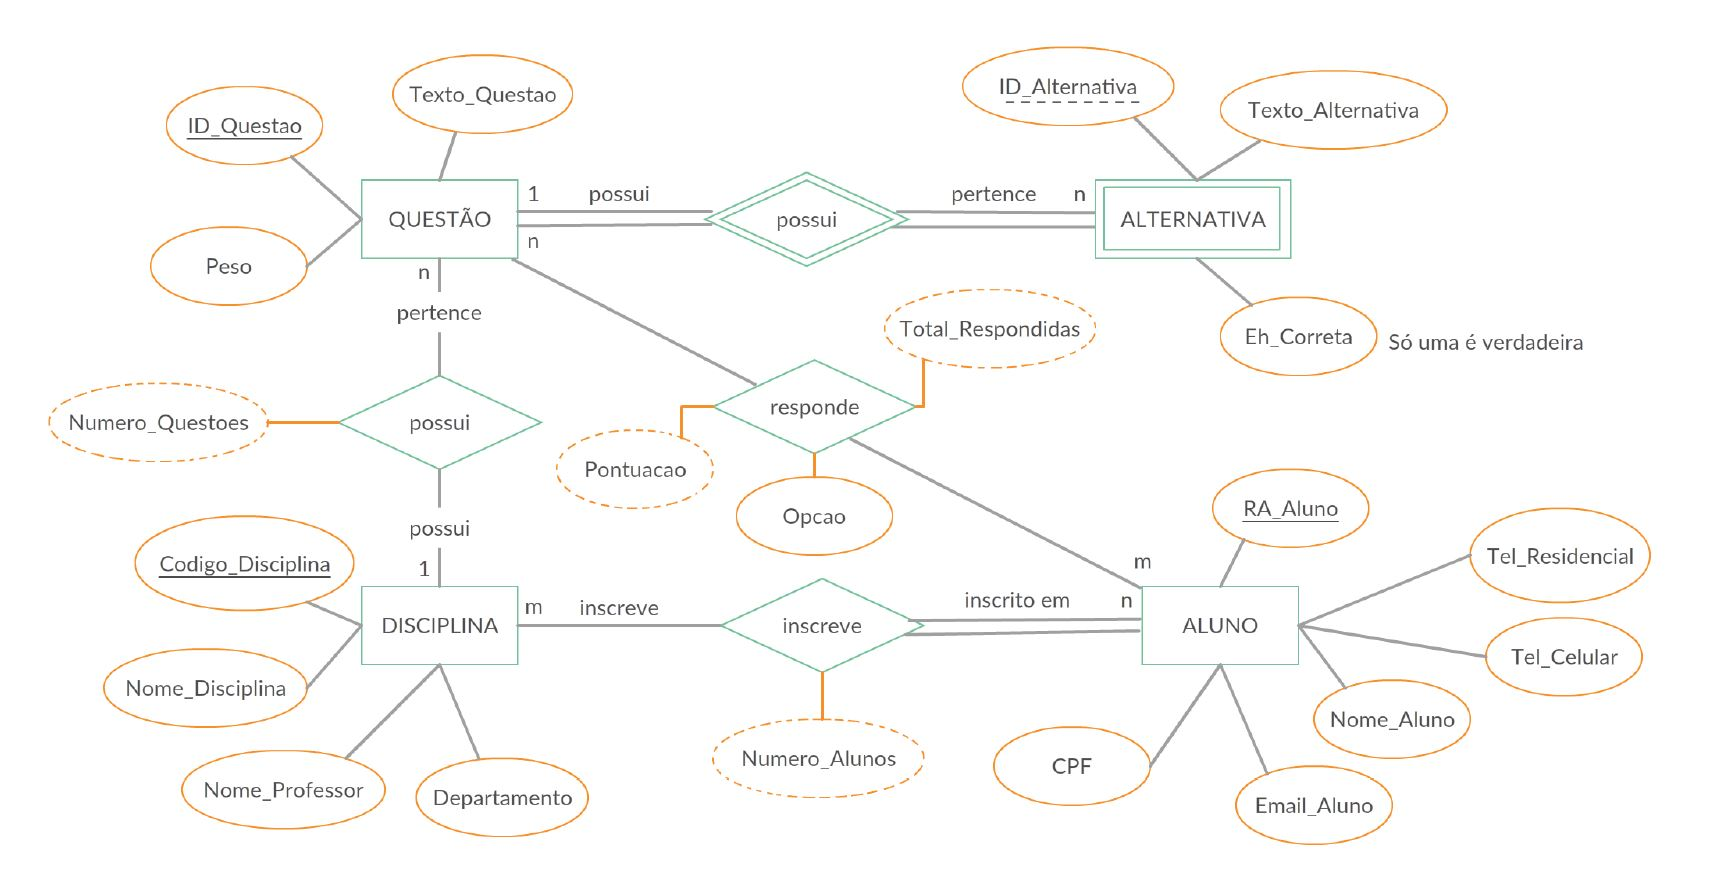
\includegraphics[width=\linewidth]{diagramaProjeto.jpg}
    \caption{MER Completo}
    \label{fig:DERcompleto}
\end{figure}
\end{center}

\subsection{Tipos-Entidade}

O sistema de Banco de Questões possui 4 tipos-entidade: {\texttt{Disciplina}}, {\texttt{Aluno}}, {\texttt{Questão}} e {\texttt{Alternativa}}. Notaremos no decorrer da próxima seção que todos os atributos são atômicos (simples) e monovalorados.

\subsection{Atributos dos Tipos-Entidade} \label{atributos_entidades}

Nesta subseção serão descritos todos os tipos-entidade, junto com os atributos que os caracterizam.

\vspace{0.5cm}
\begin{center}
    \texttt{DISCIPLINA}
\end{center}

\hspace{6}O tipo-entidade {\texttt{Disciplina}} é um objeto de existência conceitual e contém os atributos: {\texttt{Codigo\_Disciplina}}, {\texttt{Nome\_Disciplina}}, {\texttt{Departamento}} e {\texttt{Nome\_Professor}}. O atributo {\texttt{Codigo\_Disciplina}} é único e identifica o tipo-entidade. Também podemos identificar a disciplina pelo atributo {\texttt{Nome\_Disciplina}}, entretanto este não é garantidamente único, podem existir disciplinas com o mesmo nome, lecionadas por diferentes professores.\\

O atributo {\texttt{Departamento}} é utilizado para armazenar o nome do departamento em que determinada \texttt{Disciplina} é lecionada. O nome de quem leciona determinada \texttt{Disciplina} é armazenado pelo atributo {\texttt{Nome\_Professor}}. Abaixo será possível identificar as especificidades de cada atributo. \\

\begin{itemize}
    \item {\texttt{Codigo\_Disciplina}}: valor inteiro, auto incremental, chave primária, restrição obrigatório
    \item {\texttt{Nome\_Disciplina}}: string de 255 caracteres, restrição obrigatório
    \item {\texttt{Nome\_Professor}}: string de 255 caracteres, restrição obrigatório
    \item {\texttt{Departamento}}: string de 255 caracteres, restrição obrigatório
\end{itemize}

\vspace{0.5cm}
\begin{center}
    \texttt{ALUNO}
\end{center}

O tipo-entidade {\texttt{Aluno}} é um objeto de existência física e contém os atributos: {\texttt{RA\_Aluno}}, {\texttt{Nome\_Aluno}}, {\texttt{CPF}}, {\texttt{Email\_Aluno}}, {\texttt{Tel\_Celular} e \texttt{Tel\_Residencial}}. O atributo {\texttt{RA\_Aluno}} é único e identifica o tipo-entidade. É importante ressaltar este identificador é o RA\_Aluno do aluno. Também é possível utilizar o atributo {\texttt{Nome\_Aluno}} para encontrar determinado aluno, entretanto este não é um identificador único, visto que pode existir mais de um aluno com o mesmo nome.\\

O atributo {\texttt{CPF}} também é único, todavia neste caso não é utilizado para identificar um \texttt{Aluno}. Os atributos {\texttt{Email\_Aluno}}, {\texttt{Tel\_Celular} e \texttt{Tel\_Residencial}} servem para armazenar informações de contato sobre determinado \texttt{Aluno}. Abaixo será possível identificar as especificidades de cada atributo.\\

\begin{itemize}
    \item {\texttt{RA\_Aluno}}: valor inteiro, chave primária, restrição obrigatório
    \item {\texttt{Nome\_Aluno}}: string de 255 caracteres, restrição obrigatório
    \item \texttt{CPF}: string de 14 caracteres, restrição obrigatório e único
    \item \texttt{Email\_Aluno}: string de 50 caracteres, restrição obrigatório e único
    \item \texttt{Tel\_Celular}: string de 15 caracteres, restrição obrigatório
    \item \texttt{Tel\_Residencial}: string de 14 caracteres
\end{itemize}

\vspace{0.5cm}
\begin{center}
    \texttt{QUESTÃO}
\end{center}

O tipo-entidade \texttt{Questão} é um objeto de existência conceitual e contém os atributos: \texttt{ID\_Questão},  \texttt{Texto\_Questão} e \texttt{Peso}. O atributo \texttt{ID\_Questão} é único e identifica o tipo-entidade. Já o atributo \texttt{Texto\_Questão} contém o texto da questão que será apresentada ao aluno. Por último, o atributo \texttt{Peso} serve para mostrar o quanto vale cada questão e para o auxiliar no cálculo da pontuação do \texttt{Aluno}. Neste projeto, o Peso sempre será 1, ou seja, cada questão sempre valerá 1 ponto. Abaixo será possível identificar as especificidades de cada atributo.\\

\begin{itemize}
    \item \texttt{ID\_Questão}: valor inteiro, serial, chave primária, restrição obrigatório
    \item \texttt{Texto\_Questão}: texto, restrição obrigatório
    \item \texttt{Peso}: valor inteiro, restrição obrigatório
\end{itemize}

\vspace{0.5cm}
\begin{center}
    \texttt{ALTERNATIVA}
\end{center}

O tipo-entidade \texttt{Alternativa} é um objeto de existência conceitual, além de ser um tipo-entidade fraca, logo, sua existência depende de sua participação no tipo-relacionamento com o tipo-entidade \texttt{Questão} . O tipo-entidade \texttt{Alternativa} contém os atributos: \texttt{ID\_Alternativa}, \texttt{Texto\_Alternativa} e \texttt{Eh\_Correta}. O atributo \texttt{ID\_Alternativa} é uma chave parcial e identifica o tipo-entidade em conjunto com o atributo \texttt{ID\_Questão} do tipo-entidade \texttt{Questão}, visto que se trata de um tipo-entidade fraca. O atributo \texttt{Texto\_Alternativa}, por sua vez, é responsável por armazenar o texto da alternativa, ou seja, uma possível resposta.\\

O atributo \texttt{Eh\_Correta} é responsável por identificar se determinada alternativa está correta ou não. Uma alternativa precisa corresponder a uma determinada \texttt{Questão}, e apenas uma alternativa é correta dentre as alternativas de uma questão. Neste projeto, todas as questões possuem apenas quatro alternativas. Abaixo será possível identificar as especificidades de cada atributo. \\

\begin{itemize}
    \item \texttt{ID\_Alternativa}: valor inteiro, serial, chave parcial (ID\_Questão e ID\_Alternativa), restrição obrigatório
    \item \texttt{Texto\_Alternativa}: texto, restrição obrigatório
    \item \texttt{Eh\_Correta}: tupla ('Não', 'Sim'), restrição obrigatório
\end{itemize}

\subsection{Atributos Calculados}

O atributo {\texttt{Total\_Respondidas}} é um atributo calculado e corresponde ao número total de questões respondidas pelo aluno. O atributo {\texttt{Pontuação}} também calculado e é obtido a cada questão que o aluno responde corretamente. É importante ressaltar que um aluno não perde pontos caso responda incorretamente determinada questão. Este atributo pode ajudar tanto o aluno, quanto o professor, através dele ambos podem acompanhar o nível de aprendizado. Ambos estes atributos são gerados pelo tipo-relacionamento \texttt{ALUNO responde QUESTÃO}.\\

O atributo \texttt{Número\_Questões} é gerado através do tipo-relacionamento \texttt{DISCIPLINA possui QUESTÃO} e é responsável por armazenar o número de Questões existentes em uma determinada \texttt{Disciplina}. Por último, o atributo \texttt{Numero\_Alunos} é gerado pelo tipo-relacionamento \texttt{DISCIPLINA inscreve ALUNO} e é responsável por armazenar o número de \texttt{Alunos} existentes em uma determinada \texttt{Disciplina}.\\

\subsection{Tipos-Relacionamento}

\vspace{0.5cm}
\begin{center}
    \texttt{{ALUNO \texttt{responde} QUESTÃO}}
\end{center}

O tipo-entidade {\texttt{Aluno}} é responsável por responder questões do tipo-entidade \texttt{Questão}. Logo, o papel do tipo-relacionamento estabelecido entre eles é representado por responde. O tipo-relacionamento tem cardinalidade N:M, visto que um \texttt{Aluno} pode responder N Questões, e uma Questão é respondida por M \texttt{Alunos}.\\

O tipo-relacionamento \texttt{{ALUNO responde QUESTÃO}} possui o atributo \texttt{Opção}, além dos atributos calculados \texttt{Total\_Respondidas} e \texttt{Pontuação}. O atributo \texttt{Opção} é responsável por armazenar qual foi a Opção respondida pelo \texttt{Aluno}.

\begin{center}
\centering
\begin{figure}[h]
    \centering
    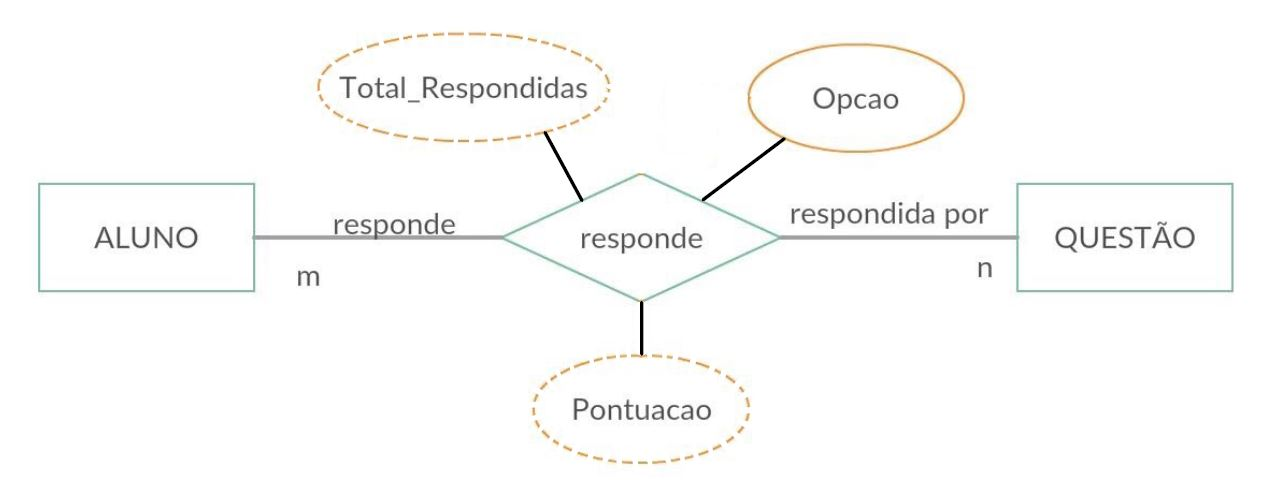
\includegraphics[width=\linewidth]{alunoQuestao.jpg}
    \caption{ALUNO responde QUESTÃO}
    \label{fig:alunoQuestao}
\end{figure}
\end{center}

\begin{center}
    \texttt{DISCIPLINA \texttt{inscreve} ALUNO}
\end{center}

O papel do tipo-relacionamento entre os tipo-entidades \texttt{Disciplina} e {\texttt{Aluno}} é representado por inscreve, visto que N \texttt{Alunos} podem se inscrever em uma \texttt{Disciplina}, e um \texttt{Aluno} pode estar inscrito em M \texttt{Disciplinas}. Deste modo, podemos concluir que a cardinalidade deste tipo-relacionamento é 1:N. Além disso, este tipo-relacionamento possui o atributo calculado {\texttt{Numero\_Alunos}}.\\

A existência do tipo-entidade \texttt{Disciplina} depende de sua participação em um tipo-relacionamento com o do tipo-entidade  {\texttt{Aluno}}. Logo, se trata de uma restrição de participação total, uma \texttt{Disciplina} existirá apenas caso hajam \texttt{Alunos} inscritos.\\

\begin{center}
\begin{figure}[h]
    \centering
    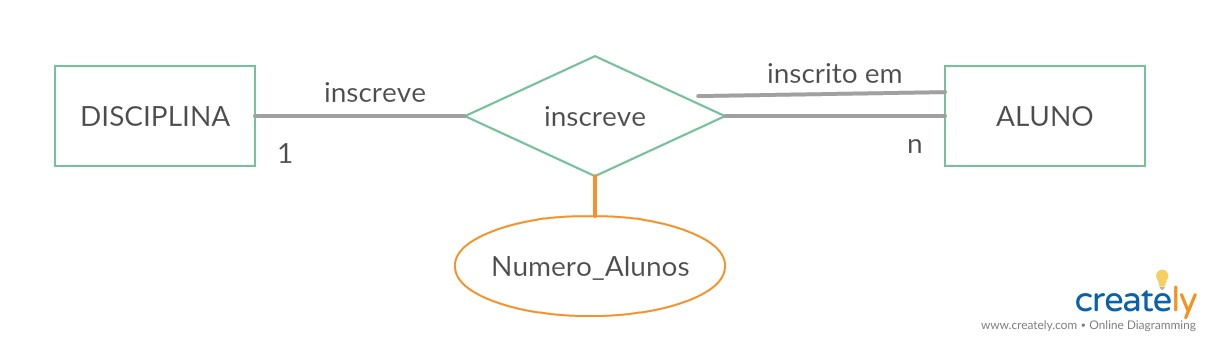
\includegraphics[width=\linewidth]{disciplinaAluno.jpg}
    \caption{DISCIPLINA inscreve ALUNO}
    \label{fig:disciplinaAluno}
\end{figure}
\end{center}

\pagebreak
\vspace{0.5cm}
\begin{center}
    \texttt{DISCIPLINA \texttt{possui} QUESTÃO}
\end{center}

O papel do tipo-relacionamento entre os tipo-entidades \texttt{Disciplina} e \texttt{Questão} é representado por possui, visto que uma \texttt{Disciplina}, pode possuir N Questões, e uma QUESTÃO pertence apenas a uma DISCIPLINA. Deste modo, podemos concluir que a cardinalidade deste tipo-relacionamento é 1:N. Além disso, este é o tipo-relacionamento que possui o atributo calculado \texttt{Numero\_Questoes}.\\

\begin{center}
\begin{figure}[h]
    \centering
    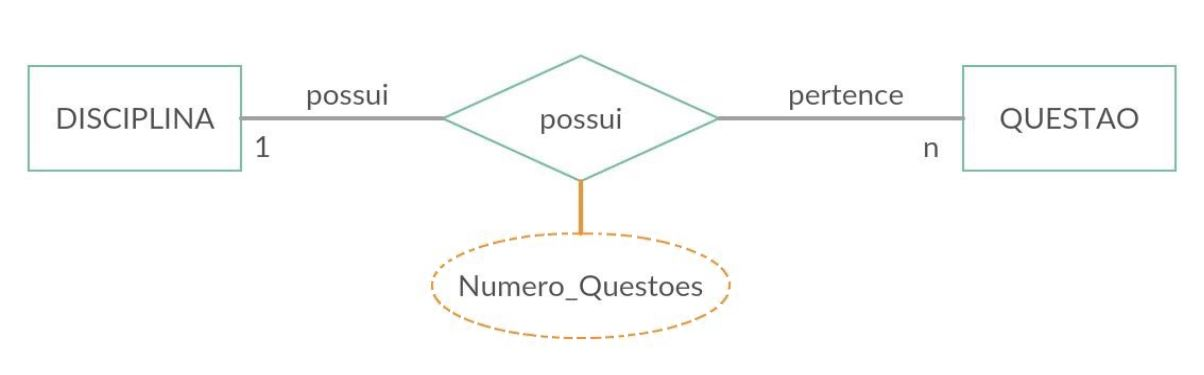
\includegraphics[width=\linewidth]{disciplinaQuestao.jpg}
    \caption{DISCIPLINA possui QUESTÃO}
    \label{fig:disciplinaQuestao}
\end{figure}
\end{center}

\begin{center}
    \texttt{QUESTÃO \texttt{possui} ALTERNATIVA}
\end{center}

O tipo-relacionamento entre os tipo-entidades \texttt{Questão} e \texttt{Alternativa} é representado por possui, visto que uma Questão possui N Alternativas. Do mesmo modo, N Alternativas pertencem à uma Questão. Logo, concluímos que a cardinalidade do tipo-relacionamento é 1:N. Ressaltando, neste projeto N sempre será igual a quatro.\\

A existência do tipo-entidade \texttt{Questão} depende de sua participação em um tipo-relacionamento com o do tipo-entidade  {\texttt{Alternativa}}. Logo, se trata de uma restrição de participação total, só existe se uma Questão possuir Alternativa(s).\\

O tipo-entidade \texttt{Alternativa} é fraco, logo sua existência depende de sua participação no tipo-relacionamento com o tipo-entidade \texttt{Questão}, que a identifica. Uma Alternativa existirá apenas caso exista uma Questão correspondente.\\

\begin{center}
\begin{figure}[h]
    \centering
    
\includegraphics[width=\linewidth]{questaoAlternativa.jpg}
    \caption{QUESTÃO possui ALTERNATIVA}
    \label{fig:questaoAlternativa}
\end{figure}
\end{center}

\pagebreak
\subsection{Requisitos de Dados}

Os Requisitos de Dados representam as consultas, inserções, modificações, remoções, agregações que o projeto deve ser capaz de executar. A seguir será possível visualizar alguns exemplos:

\vspace{0.5cm}
\begin{center}
    \texttt{INSERÇÕES}
\end{center}
\begin{enumerate}
    \item O sistema deve permitir o cadastro de um \texttt{Aluno} em uma \texttt{Disciplina} a partir dos atributos do tipo-entidade \texttt{Aluno}
    \item O sistema deve permitir o cadastro de uma \texttt{Disciplina} a partir dos atributos do tipo-entidade \texttt{Disciplina}
    \item O sistema deve permitir o cadastro de uma Questão de uma determinada \texttt{Disciplina} a partir dos atributos do tipo-entidade Questão
    \item O sistema deve permitir a adição de Alternativas de uma determinada Questão a partir dos atributos do tipo-entidade Alternativa
\end{enumerate}

\vspace{0.5cm}
\begin{center}
    \texttt{BUSCAS}
\end{center}
\begin{enumerate}
    \item O sistema deve permitir a busca de um Aluno pertencente à uma \texttt{Disciplina}
        \begin{itemize}
            \item Atributo(s) de visualização do resultado: {\texttt{RA\_Aluno}}, {\texttt{Nome\_Aluno}}
            \item Atributo(s) de busca (ou de condições/filtros): {\texttt{RA\_Aluno}} ou {\texttt{Nome\_Aluno}}, \texttt{Codigo\_Disciplina}
        \end{itemize}
    \item O sistema deve permitir busca de Questões a partir de uma palavra chave
        \begin{itemize}
            \item Atributo(s) de visualização do resultado: \texttt{ID\_Questão}, \texttt{Texto\_Questão}, \texttt{Codigo\_Disciplina}
            \item Atributo(s) de busca (ou de condições/filtros): palavra chave ('\%palavra-chave\%')
        \end{itemize}
    \item O sistema deve permitir busca de Questões de uma determinada \texttt{Disciplina}
        \begin{itemize}
            \item Atributo(s) de visualização do resultado: \texttt{ID\_Questão}, \texttt{Texto\_Questão}
            \item Atributo(s) de busca (ou de condições/filtros): \texttt{Codigo\_Disciplina}
        \end{itemize}
    \item O sistema deve permitir busca de uma \texttt{Disciplina} à partir de seu código 
        \begin{itemize}
            \item Atributo(s) de visualização do resultado: atributos da \texttt{Disciplina} encontrada
            \item Atributo(s) de busca (ou de condições/filtros): \texttt{Codigo\_Disciplina}
        \end{itemize}
    % CÁLCULOS
    \item O sistema deve permitir o cálculo do número de \texttt{Alunos} inscritos por \texttt{Disciplina}
        \begin{itemize}
            \item Atributo(s) de visualização do resultado: número de alunos
            \item Atributo(s) de cálculo: \texttt{Codigo\_Disciplina}
        \end{itemize}
    \item O sistema deve permitir o cálculo do número de Questões respondidas por um Aluno
        \begin{itemize}
            \item Atributo(s) de visualização do resultado: número de questões respondidas
            \item Atributo(s) de cálculo: obtido através do tipo-relacionamento \texttt{ALUNO responde QUESTÃO}
        \end{itemize}
    \item O sistema deve permitir o cálculo da pontuação do Aluno
        \begin{itemize}
            \item Atributo(s) de visualização do resultado: pontuação do Aluno
            \item Atributo(s) de cálculo: peso da questão e número de acertos
        \end{itemize}
    \item O sistema deve permitir o cálculo do número de Alunos e do número de Questões de uma determinada \texttt{Disciplina}
    % AGREGAÇÃO
    \item O sistema deve permitir a visualização de todas as alternativas de uma determinada questão
    \item O sistema deve permitir a visualização de todos os alunos em uma determinada \texttt{Disciplina}
\end{enumerate}


\vspace{0.5cm}
\begin{center}
    \texttt{MODIFICAÇÕES}
\end{center}
\begin{enumerate}
    \item O sistema deve permitir a alteração de dados da \texttt{Disciplina}
    \item O sistema deve permitir a alteração de dados do Aluno
\end{enumerate}

\vspace{0.5cm}
\begin{center}
    \texttt{REMOÇÕES}
\end{center}
\begin{enumerate}
    \item O sistema deve permitir a remoção de Questões
    \item O sistema deve permitir a remoção de \texttt{Alunos}
\end{enumerate}


\pagebreak

\subsection{Tabelas de Metadados}
A tabela de metadados contém basicamente um resumo de cada tipo-entidade, com seu nome e atributos, junto com o tipo e restrição de cada atributo.

% Table generated by Excel2LaTeX from sheet 'Sheet1'
\begin{table}[h]
  \centering
  \caption{Tipo-Entidade Aluno}
    \begin{tabular}{|c|c|l|l|l|}
    \toprule\hline
    \multicolumn{2}{|c|}{\textbf{Tipo-Entidade}} & \textbf{Atributo} & \textbf{Tipo} & \textbf{Restrição} \\\hline
    \midrule
    \multicolumn{2}{|c|}{\texttt{Aluno}} & \texttt{RA\_Aluno} & Identificador & Obrigatório \\
    \midrule
    \multicolumn{2}{|c|}{} & \texttt{Nome\_Aluno} & Monovalorado & Obrigatório \\
    \midrule
    \multicolumn{2}{|c|}{} & \texttt{CPF}   & Monovalorado & Obrigatório e Único \\
    \midrule
    \multicolumn{2}{|c|}{} & \texttt{Email\_Aluno} & Monovalorado & Obrigatório e Único \\
    \midrule
    \multicolumn{2}{|c|}{} & \texttt{Tel\_Celular} & Monovalorado & Obrigatório \\
    \midrule
    \multicolumn{2}{|c|}{} & \texttt{Tel\_Residencial} & Monovalorado & Opcional \\
    \bottomrule\hline
    \end{tabular}%
  \label{tab:meta_aluno}%
\end{table}%

% Table generated by Excel2LaTeX from sheet 'Sheet1'
\begin{table}[h]
  \centering
  \caption{Tipo-Entidade Disciplina}
    \begin{tabular}{|cc|l|l|l|}
    \toprule\hline
    \multicolumn{2}{|c|}{\textbf{Tipo-Entidade}} & \textbf{Atributo} & \textbf{Tipo} & \textbf{Restrição} \\\hline
    \midrule
    \multicolumn{2}{|c|}{\multirow{\texttt{Disciplina}}} & \texttt{Codigo\_Disciplina} & Identificador & Obrigatório \\
    \multicolumn{2}{|c|}{} & \texttt{Nome\_Disciplina} & Monovalorado & Obrigatório \\
    \multicolumn{2}{|c|}{} & \texttt{Nome\_Professor} & Monovalorado & Obrigatório \\
    \multicolumn{2}{|c|}{} & \texttt{Departamento} & Monovalorado & Obrigatório \\
    \bottomrule\hline
    \end{tabular}%
  \label{tab:addlabel}%
\end{table}%

% Table generated by Excel2LaTeX from sheet 'Sheet1'
\begin{table}[h]
  \centering
  \caption{Tipo-Entidade Questão}
    \begin{tabular}{|c|c|l|l|l|}
    \toprule\hline
    \multicolumn{2}{|c|}{\textbf{Tipo-Entidade}} & \textbf{Atributo} & \textbf{Tipo} & \textbf{Restrição} \\\hline
    \midrule
    \multicolumn{2}{|c|}{\texttt{Questão}} & \texttt{ID\_Questao} & Identificador & Obrigatório \\
    \midrule
    \multicolumn{2}{|c|}{} & \texttt{Texto\_Questao} & Monovalorado & Obrigatório \\
    \midrule
    \multicolumn{2}{|c|}{} & \texttt{Peso} & Monovalorado & Obrigatório, Peso = 1 \\
    \midrule
    \bottomrule\hline
    \end{tabular}%
  \label{tab:meta_questao}%
\end{table}%

% Table generated by Excel2LaTeX from sheet 'Sheet1'
\begin{table}[h]
  \centering
  \caption{Alternativa}
    \begin{tabular}{|c|c|l|l|l|}
    \toprule\hline
    \multicolumn{2}{|c|}{\textbf{Tipo-Entidade}} & \textbf{Atributo} & \textbf{Tipo} & \textbf{Restrição} \\\hline
    \midrule
    \multicolumn{2}{|c|}{\texttt{Alternativa}} & \texttt{ID\_Alternativa} & Chave Parcial & Obrigatório \\
    \midrule
    \multicolumn{2}{|c|}{} & \texttt{Texto\_Alternativa} & Monovalorado & Obrigatório \\
    \midrule
    \multicolumn{2}{|c|}{} & \texttt{Eh\_Correta} & Monovalorado & Obrigatório, 'Não' ou 'Sim' \\
    \midrule
    \bottomrule\hline
    \end{tabular}%
  \label{tab:meta_alternativa}%
\end{table}%
\pagebreak

\section{Projeto Lógico}

O projeto lógico consiste no mapeamento do esquema desenvolvido na seção \texttt{Projeto Conceitual}, além da aplicação das regras de normalização que são \texttt{1FN}, \texttt{2FN} e \texttt{3FN}.

\subsection{Mapeamento}

Inicialmente os tipo-entidade forte \texttt{Questão}, \texttt{Disciplina} e \texttt{Aluno} foram mapeados. Para isso utilizamos n colunas, uma para cada atributo. Por conseguinte, foram obtidas as seguintes relações:

\begin{Verbatim}[commandchars=+\[\]]
    Questao (+underline[id_questao], texto_questao, peso)
\end{Verbatim}
\begin{Verbatim}[commandchars=+\[\]]
    Disciplina (+underline[codigo_disciplina], nome_disciplina,
    departamento, nome_professor)
\end{Verbatim}
\begin{Verbatim}[commandchars=+\[\]]
    Aluno (+underline[ra_aluno], cpf, nome_aluno, email_aluno,
    tel_residencial, tel_celular)
\end{Verbatim}

Em seguida, o tipo-entidade fraca \texttt{Alternativa} foi mapeado, criando uma tabela própria com chave primária igual ao conjunto dos dois tipos-entidade envolvidos: \texttt{Questão} e \texttt{Alternativa}. Por conseguinte, foi obtida a seguinte relação:

\begin{Verbatim}[commandchars=+\[\]]
    Alternativa (+underline[id_questao], +underline[id_alternativa], texto_alternativa, 
    eh_correta)
        id_questao referencia Questao
\end{Verbatim}

Em seguida, foram mapeados os tipos-relacionamento 1:n.

Para o relacionamento \texttt{DISCIPLINA possui QUESTÃO}, foi utilizada a técnica de adição de coluna, criando um atributo no lado n, atualizando o mapeamento da \texttt{Questão}:

\begin{Verbatim}[commandchars=+\[\]]
    Questao (+underline[id_questao], texto_questao, peso,
    codigo_disciplina)
        codigo_disciplina referencia Disciplina
\end{Verbatim}

Além disso, foi inserido o atributo calculado Numero\_Questoes, atualizando o mapeamento da \texttt{Disciplina}:

\begin{Verbatim}[commandchars=+\[\]]
    Disciplina (+underline[codigo_disciplina], nome_disciplina,
    departamento, nome_professor, numero_questoes)
\end{Verbatim}

Para tipo-relacionamento \texttt{QUESTÃO possui ALTERNATIVA}, mapeamos novamente através da técnica de adição de coluna, criando um atributo do lado n. Entretanto, se trata de uma entidade fraca, logo, a relação permaneceu igual:

\begin{Verbatim}[commandchars=+\[\]]
    Alternativa (+underline[id_questao], +underline[id_alternativa], texto_alternativa, 
    eh_correta)
        id_questao referencia Questao
\end{Verbatim}

Por fim, foram mapeados os tipos-relacionamento n:m.

Para o tipo-relacionamento \texttt{ALUNO responde QUESTÃO}, foi utilizada a técnica de criação de uma tabela própria, obtendo a seguinte relação:

\begin{Verbatim}[commandchars=+\[\]]
    Responde (+underline[ra_aluno], +underline[id_questao], opcao)
        ra_aluno referencia Aluno
        id_questao referencia Questao
\end{Verbatim}

Além disso, foram inseridos os atributos calculados Total\_Respondidas e Pontuacao, atualizando o mapeamento do \texttt{Aluno}:

\begin{Verbatim}[commandchars=+\[\]]
    Aluno (+underline[ra_aluno], cpf, nome_aluno, email_aluno, 
    tel_residencial, tel_celular, total_respondidas, pontuacao)
\end{Verbatim}

Para o tipo-relacionamento \texttt{DISCIPLINA inscreve ALUNO}, foi utilizada a técnica de criação de tabela própria, obtendo a seguinte relação:

\begin{Verbatim}[commandchars=+\[\]]
    Aluno_Disciplina (+underline[ra_aluno], +underline[codigo_disciplina])
        ra_aluno referencia Aluno
        codigo_disciplina referencia Disciplina
\end{Verbatim}

Além disso, foi inserido o atributo calculado Numero\_Alunos, atualizando o mapeamento da \texttt{Disciplina}:

\begin{Verbatim}[commandchars=+\[\]]
    Disciplina (+underline[codigo_disciplina], nome_disciplina,
    departamento, nome_professor, numero_questoes, numero_alunos)
\end{Verbatim}

Para melhor visualização, mostraremos a seguir todas as relações criadas:\\

\begin{Verbatim}[commandchars=+\[\]]
    Disciplina (+underline[codigo_disciplina], nome_disciplina,
    departamento, nome_professor, numero_questoes, numero_alunos)
\end{Verbatim}

\begin{Verbatim}[commandchars=+\[\]]
    Aluno (+underline[ra_aluno], cpf, nome_aluno, email_aluno, 
    tel_residencial, tel_celular, total_respondidas, pontuacao)
\end{Verbatim}

\begin{Verbatim}[commandchars=+\[\]]
    Aluno_Disciplina (+underline[ra_aluno], +underline[codigo_disciplina])
        ra_aluno referencia Aluno
        codigo_disciplina referencia Disciplina
\end{Verbatim}

\begin{Verbatim}[commandchars=+\[\]]
    Questao (+underline[id_questao], texto_questao, peso,
    codigo_disciplina)
        codigo_disciplina referencia Disciplina
\end{Verbatim}

\begin{Verbatim}[commandchars=+\[\]]
    Alternativa (+underline[id_questao], +underline[id_alternativa], texto_alternativa, 
    eh_correta)
        id_questao referencia Questao
\end{Verbatim}

\begin{Verbatim}[commandchars=+\[\]]
    Responde (+underline[ra_aluno], +underline[id_questao], opcao)
        ra_aluno referencia Aluno
        id_questao referencia Questao
\end{Verbatim}

É importante ressaltar que mapeamento se encontra na 1FN, visto que todos os atributos são atômicos e monovalorados, ou seja, não existem atributos multivalorados. Também podemos dizer que o mapeamento se encontra na 2FN, visto que se encontra na 1FN e não há dependência funcional parcial.\\

Por fim, também podemos dizer que os mapeamentos se encontram na 3FN, visto que estão na 1FN, 2FN e nenhum atributo não chave depende de atributos não chave.

\subsection{Diagrama Entidade Relacionamento (DER)}

Obtidas todas as relações e verificadas as normalizações, foi possível obter o diagrama completo com todas as entidades, além de setas indicando as referências às outras entidades (chaves estrangeiras).

\begin{center}
\begin{figure}[h]
    \centering
    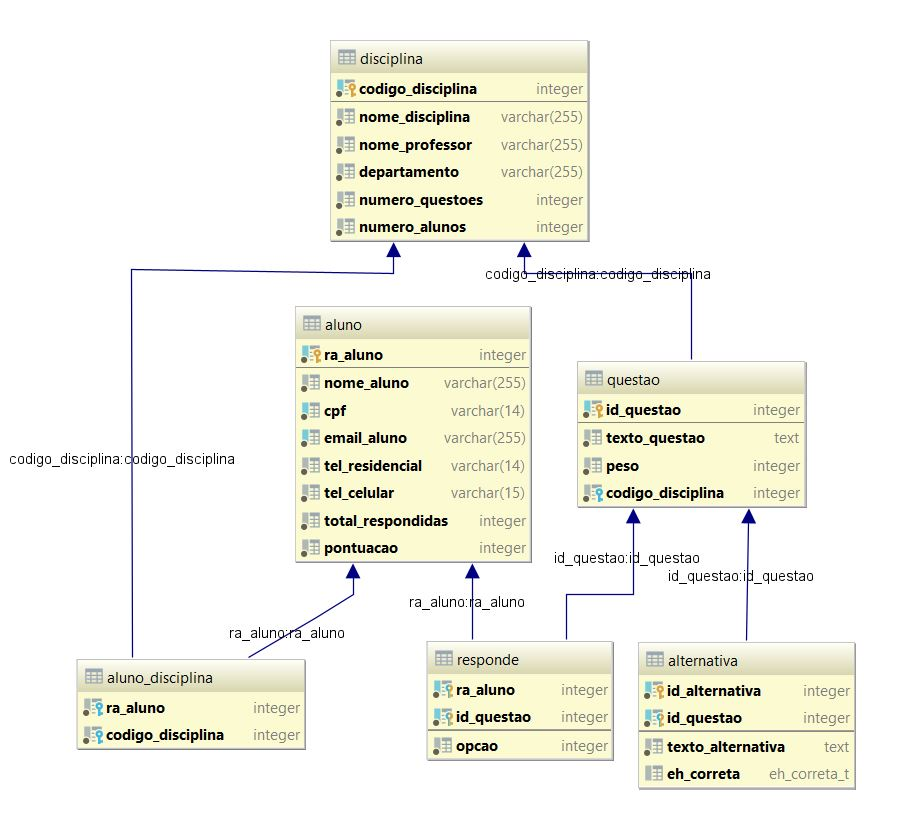
\includegraphics[width=\linewidth]{mapeamento.jpg}
    \caption{DER Completo}
    \label{fig:DERcompleto}
\end{figure}
\end{center}

\section{Projeto Físico}

O projeto físico corresponde à implementação em si do Banco de Dados Relacional. Os comandos foram criados à partir da linguagem SQL, através do Sistema de Gerenciamento de Banco de Dados (SGBD) PostgreSQL. Os scripts de criação do banco de dados se encontram anexados no arquivo \textit{esquema.sql}, e os de inserção se encontram anexados no arquivo \textit{dados.sql};

\subsection{Políticas de Restrição de Integridade}

Para a tabela \texttt{Disciplina}, temos as seguintes restrições de integridade:

\begin{itemize}
    \item {\texttt{Codigo\_Disciplina}}: NOT NULL e PRIMARY KEY
    \item {\texttt{Nome\_Disciplina}}: NOT NULL
    \item {\texttt{Nome\_Professor}}: NOT NULL
    \item {\texttt{Departamento}}: NOT NULL
    \item {\texttt{Numero\_Questoes}}: NOT NULL e DEFAULT 0
    \item {\texttt{Numero\_Alunos}}: NOT NULL, DEFAULT 0 e CHECK (Numero\_Alunos <= 20) 
\end{itemize}

Para a tabela \texttt{Aluno}, temos as seguintes restrições de integridade:

\begin{itemize}
    \item {\texttt{RA\_Aluno}}: NOT NULL e PRIMARY KEY
    \item {\texttt{Nome\_Aluno}}: NOT NULL
    \item \texttt{CPF}: NOT NULL e UNIQUE
    \item \texttt{Email\_Aluno}: NOT NULL e UNIQUE
    \item \texttt{Tel\_Celular}: NOT NULL
    \item \texttt{Tel\_Residencial}:
    \item \texttt{Total\_Respondidas}: NOT NULL e DEFAULT 0
    \item \texttt{Tel\_Pontuacao}: NOT NULL e DEFAULT 0
\end{itemize}

Para a tabela \texttt{Aluno\_Disciplina}, temos as seguintes restrições de integridade:

\begin{itemize}
    \item {\texttt{RA\_Aluno}}: NOT NULL, PRIMARY KEY, FOREIGN KEY, ON DELETE CASCADE e ON UPDATE CASCADE
    \item {\texttt{Codigo\_Disciplina}}: NOT NULL, PRIMARY KEY, FOREIGN KEY, ON DELETE CASCADE e ON UPDATE CASCADE
\end{itemize}

Para a tabela \texttt{Questao}, temos as seguintes restrições de integridade:

\begin{itemize}
    \item \texttt{ID\_Questão}: NOT NULL e PRIMARY KEY
    \item \texttt{Texto\_Questão}: NOT NULL
    \item \texttt{Peso}: NOT NULL, DEFAULT 1 e CHECK (Peso = 1)
    \item \texttt{Codigo\_Disciplina}: NOT NULL, FOREIGN KEY, ON DELETE RESTRICT e ON UPDATE CASCADE
\end{itemize}

Para a tabela \texttt{Alternativa}, temos as seguintes restrições de integridade:

\begin{itemize}
    \item \texttt{ID\_Alternativa}: NOT NULL e PRIMARY KEY
    \item \texttt{ID\_Questao}: NOT NULL, PRIMARY KEY, FOREIGN KEY, ON DELETE CASCADE e ON UPDATE CASCADE
    \item \texttt{Texto\_Alternativa}: NOT NULL
    \item \texttt{Eh\_Correta}: 'Sim' ou 'Nao'
\end{itemize}

Para a tabela \texttt{Responde}, temos as seguintes restrições de integridade:

\begin{itemize}
    \item \texttt{ID\_Alternativa}: NOT NULL e PRIMARY KEY
    \item \texttt{ID\_Questao}: NOT NULL, PRIMARY KEY, FOREIGN KEY, ON DELETE CASCADE e ON UPDATE CASCADE
    \item \texttt{Texto\_Alternativa}: NOT NULL
    \item \texttt{Eh\_Correta}: 'Sim' ou 'Nao'
\end{itemize}

\begin{itemize}
    \item \texttt{RA\_Aluno}: NOT NULL, PRIMARY KEY, FOREIGN KEY, ON DELETE CASCADE e ON UPDATE CASCADE
    \item \texttt{ID\_Questao}: NOT NULL, PRIMARY KEY, FOREIGN KEY, ON DELETE CASCADE e ON UPDATE CASCADE
    \item \texttt{Opcao}: NOT NULL
\end{itemize}

\end{document}